\documentclass[xcolor=table]{beamer}
\usepackage[table,xcdraw]{xcolor}
\usepackage[utf8]{inputenc}
\usepackage[utf8]{inputenc}
\usepackage{epigraph}
\usepackage{graphicx}
\usepackage[left=25mm,right=25mm,top=2cm,bottom=2cm]{geometry}
\usepackage{indentfirst}
\usepackage{hyperref}
\usepackage{amsmath}
\usepackage{xcolor}
\usepackage{float}
\usepackage{wrapfig}
\usepackage{subfig}
\usepackage{derivative}
\usepackage[table,xcdraw]{xcolor}
\usepackage[english, russian]{babel}
\usepackage{setspace}

\usetheme{Madrid}
\usecolortheme{default}

%------------------------------------------------------------
%This block of code defines the information to appear in the
%Title page
\title[Измерение Модуля Юнга] %optional
{Измерение Модуля Юнга
Методом Акустического
Резонанса}

%\subtitle{Начало}

\author[Аношин, Масов] 
{М.~Аношин\inst{1} \and Е. ~Масов\inst{1}}

\date[15.10.2022] 
{МФТИ, Октябрь 2022}

\begin{document}
\frame{\titlepage}

\section{Цель работы}
\begin{frame}
\frametitle{Цель работы}
    \large{\textbf{Цели работы:}}
    \begin{itemize}
        \item Исследовать явление акустического резонанса в тонком стержне.
        \item Измерить скорость распространения продольных звуковых колебаний в тонких стержнях из различных материалов и различных размеров.
        \item Измерить модули Юнга различных материалов.
    \end{itemize}
    \vspace{15}
    \large{\textbf{В работе используются:}}\\
    \begin{itemize}
        \large \normalsize{Генератор звуковых частот, частотомер, осциллограф,
                электромагнитные излучатель и приёмник колебаний, набор стержней из различных материалов.}
    \end{itemize}
\end{frame}

\begin{frame}{Теория}
    Волновое уравнение:
    $$ \frac{\partial^2 \zeta}{\partial  t^2} = u^2 \cdot \frac{\partial^2 \zeta}{\partial  x^2} $$
    
    Распространение плоской бегущей гармонической волны по стержню:
    $$ \zeta (x, t) = A\cdot cos(\omega t - kx + \phi_0) $$
    $$ \frac{\partial^2 \zeta}{\partial  t^2} = -\omega^2 \cdot A \cdot cos(\omega t - kx +\phi_0)$$
    $$ \frac{\partial^2 \zeta}{\partial  x^2} = -k^2 \cdot A \cdot cos(\omega t - kx +\phi_0)$$
    $$\frac{\partial^2 \zeta}{\partial  t^2} = \frac{\omega^2}{k^2} \cdot \frac{\partial^2 \zeta}{\partial  x^2}$$
    $$u = \frac{\omega}{k} = c$$ 
    \centering - скорость распространения волны в стержне
\end{frame}

%Теория1
\begin{frame}
\frametitle{Теория}
    \large Основной характеристикой упругих свойств твёрдого тела является его
        модуль Юнга \textbf{E}
        
    \large Если к элементу среды приложенно механическое напряжение вдоль
        оси OX (напряжение по другим осям при этом отсутствуют), то в этом элементе
        вдоль оси возникнет относительная деформация
        
    $$ \epsilon = \frac{\Delta x}{x} $$
    
    \large Напряжение в элементарной площадке S:
    \large $$ \sigma = \frac{\text{F}}{S} $$
    \large \[ \sigma = \epsilon \cdot \textbf{E}\]
\end{frame}

\begin{frame}
\frametitle{Теория}
    \begin{figure}[t]
        \centering
        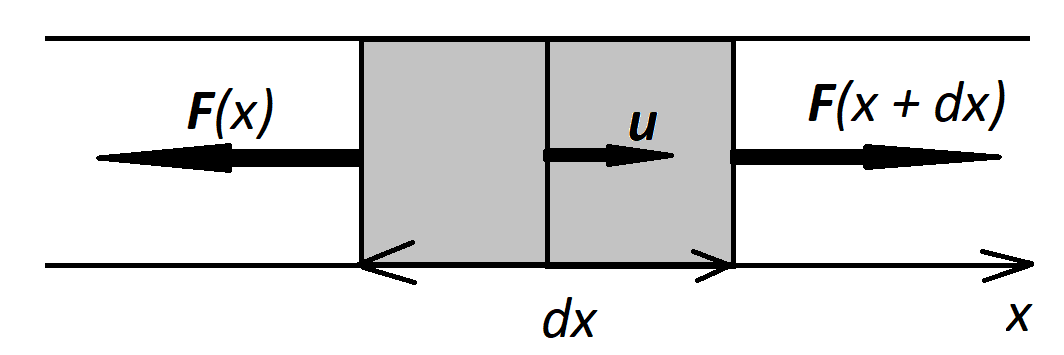
\includegraphics[width = 0.5\linewidth]{images/Wave equation.png}
        \caption{1. Иллюстрация смещения}
        \label{fig:my_label}
    \end{figure}
    \centering
    \begin{spacing}{0.1}
    \large Пусть к моменту t слой среды сместился на \zeta(x, t)\\
    \centering
    \large 
    $$dm \cdot \frac{\partial^2 \zeta}{\partial t^2} = F(x+dx) - F(x) = (\sigma_x_+_d_x - \sigma_x)S = \frac{\partial \sigma}{\partial x} \cdot Sdx$$ \\
    $$\rho \cdot S dx \cdot \frac{\partial^2 \zeta}{\partial t^2} = E \cdot S \cdot \frac{\partial^2 \zeta}{\partial x^2} \cdot dx$$ \\
    $$\frac{\partial^2 \zeta}{\partial t^2} = \frac{E}{\rho} \cdot \frac{\partial^2 \zeta}{\partial x^2} \Rightarrow c = \sqrt{\frac{E}{\rho}}$$
    \end{spacing}
\end{frame}


\begin{frame}
\frametitle{Установка}
\begin{figure}
    \centering
    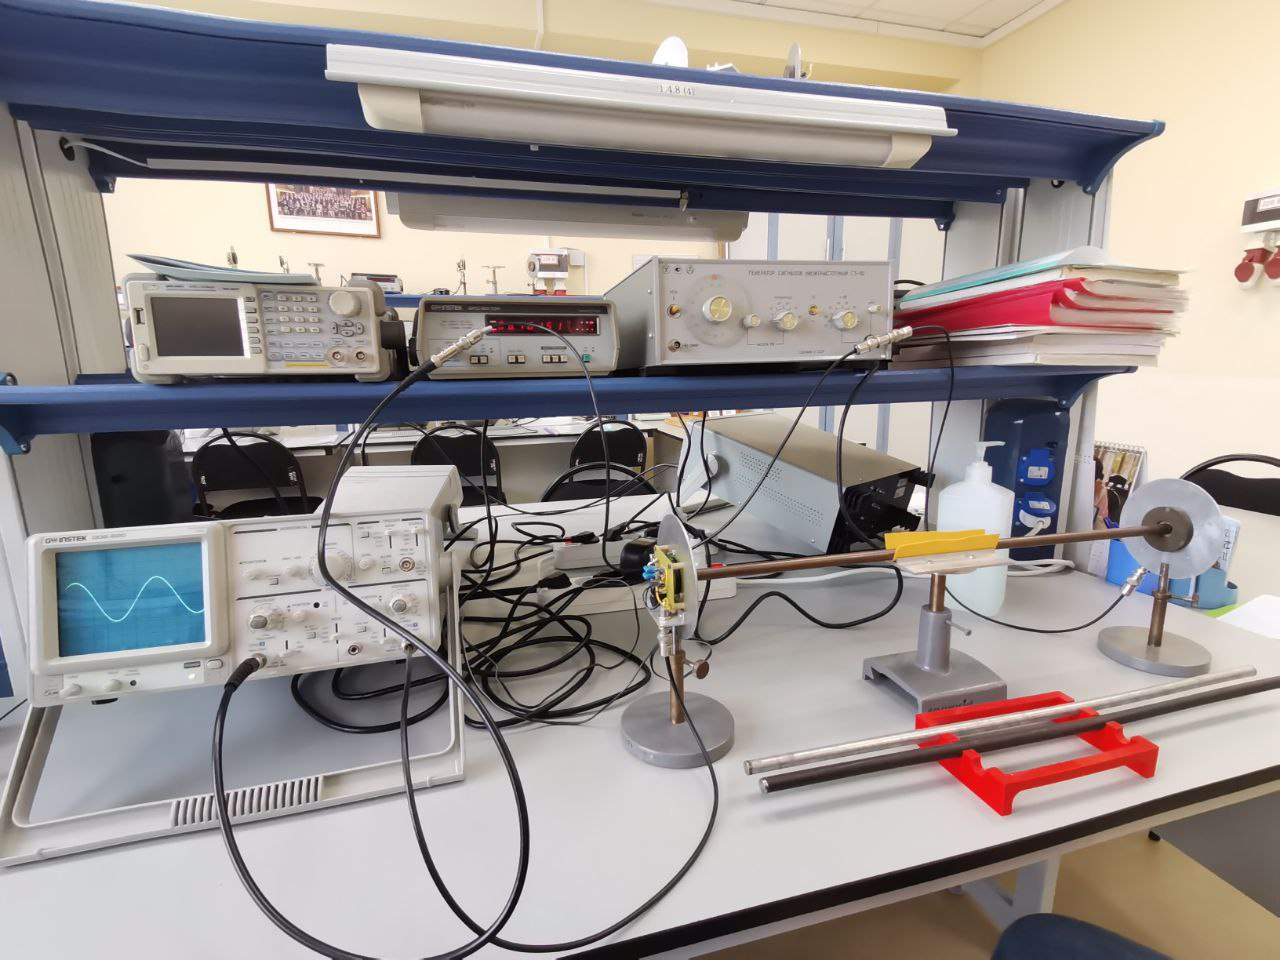
\includegraphics[scale=0.2]{images/installation.jpg}
    \caption{2. Полная фотография установки}
    \label{fig:my_label}
\end{figure}
\end{frame}

\begin{frame}
\frametitle{В установку входит:}
\begin{enumerate}
    \footnotesize
    \item Генератор звуковой частоты
    \item Частотомер
    \item Осциллограф
    \item Электромагниты (приемник и возбудитель)
\end{enumerate}
\begin{figure}
    \centering
    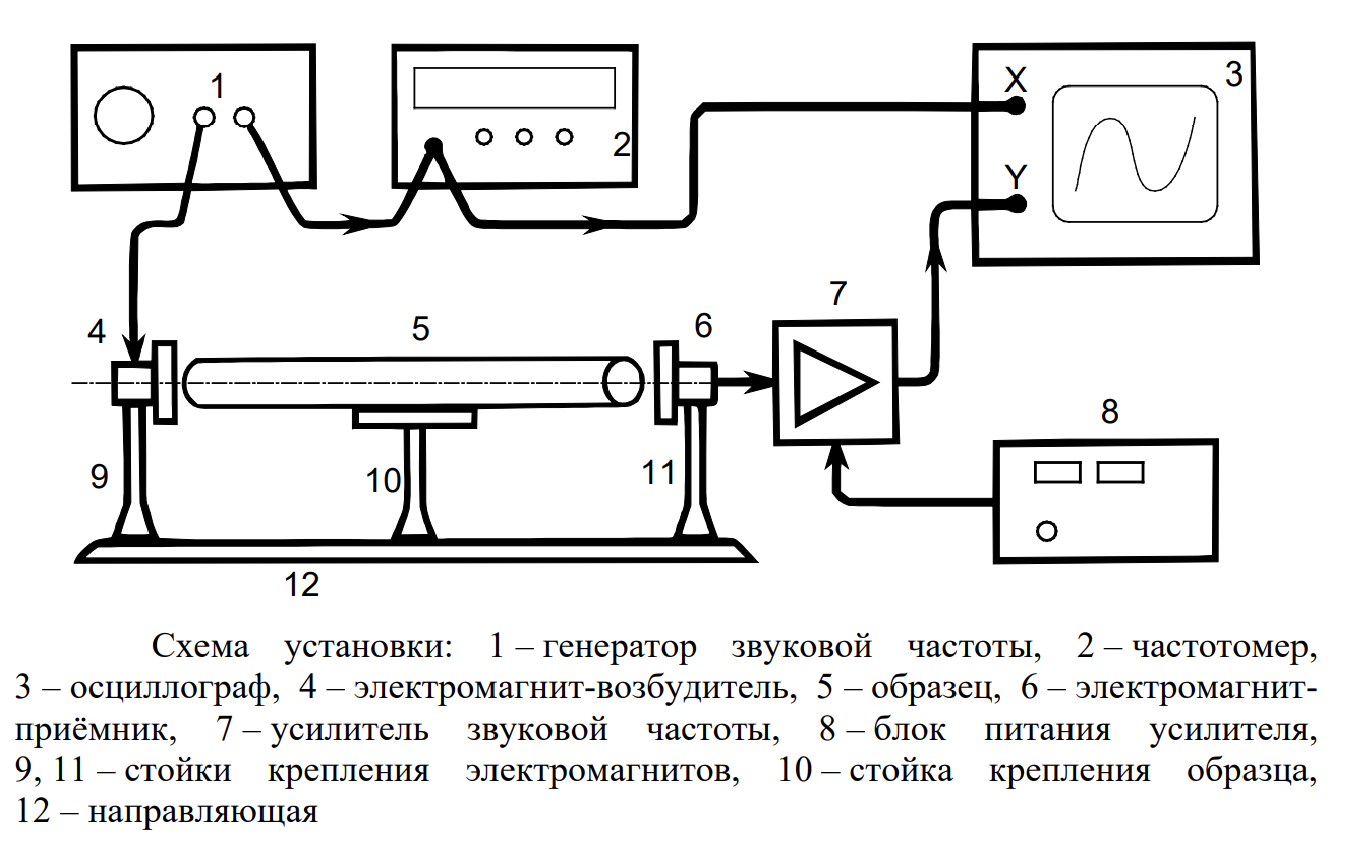
\includegraphics[scale=0.5]{images/scheme.png}
    \caption{3. Схема установки}
    \label{fig:my_label}
\end{figure}
\end{frame}

%\begin{frame}{Установка}
%    \begin{figure}
%        \centering
%        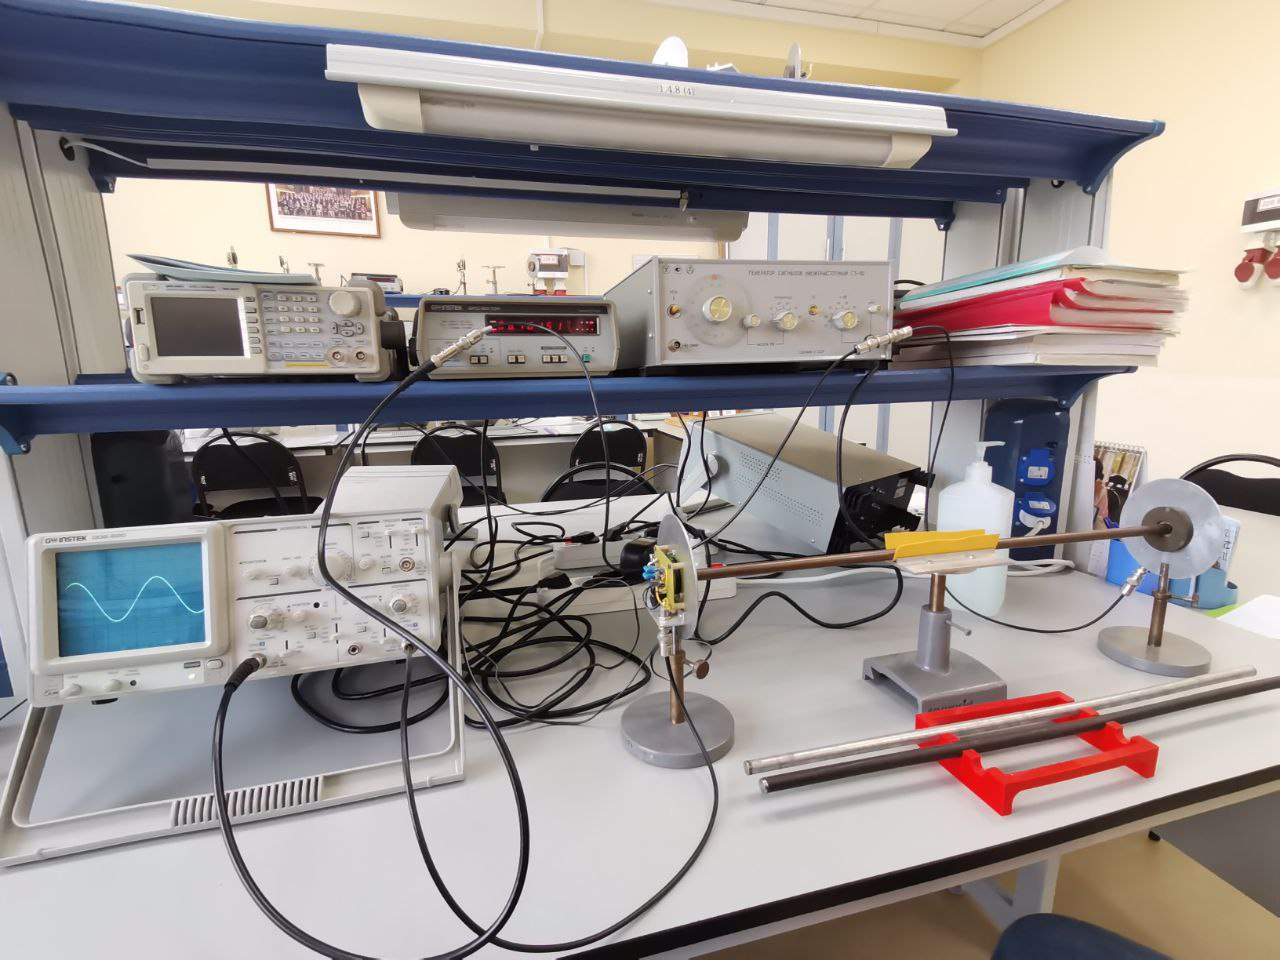
\includegraphics{images/installation.jpg}
%        \caption{4. Установка для измерений}
%        \label{fig:my_label}
%    \end{figure}
%\end{frame}

\begin{frame}
\frametitle{Генератор звуковой частоты}
\large Гвоздь программы - советский генератор
\begin{figure}
    \centering
    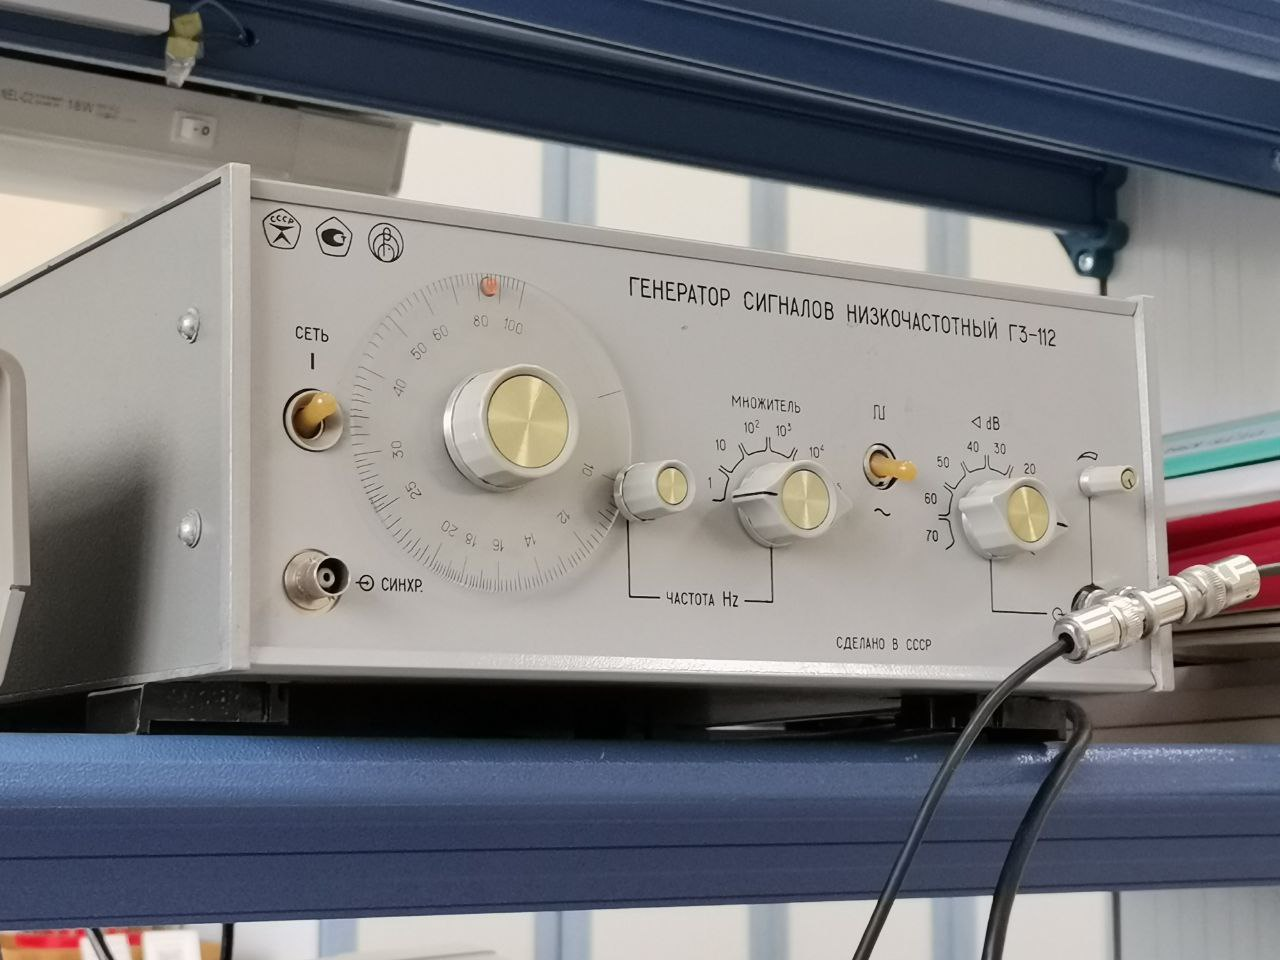
\includegraphics[scale=0.2]{images/soviet_base.jpg}
    \caption{5. Советская база}
    \label{fig:my_label}
\end{figure}
\end{frame}

\begin{frame}{Метод измерений}
    \begin{spacing}{0.25}
    $$ \zeta (x, t) = A_1\cdot cos(\omega t - kx + \phi_1) + A_2\cdot cos(\omega t + kx + \phi_2), \;\; k = \frac{2\pi}{\lambda}$$
    Координаты концов стержня не закреплены 
    $$\sigma(0) = \frac{\partial \zeta}{\partial x}\bigg|_{x=0} = 0, \;\;\; \sigma(L) = \frac{\partial \zeta}{\partial x}\bigg|_{x=L} = 0$$
    $$-kA_1\cdot cos(\omega t + \phi_1) + kA_2\cdot cos(\omega t + \phi_2) = 0$$
    $$\phi_1 = \phi_2, \;\;\; A_1 = A_2$$
    $$\zeta(x,t) = 2A\cdot cos(kx) \cdot sin(\omega t + \phi)$$
    $$\text{ищем резонанас для}\; \lambda = \frac{2L}{n} \Rightarrow f = n\frac{c}{2L}, \;\text{L - длина стержня,} \; n \; \in N$$
    \end{spacing}
\end{frame}

\begin{frame}{Показания осциллографа}
    \centering
    Фигуры Лиссажу на осциллографе при резонансе
    \begin{figure}[ht]
        \begin{minipage}{.5\textwidth}
            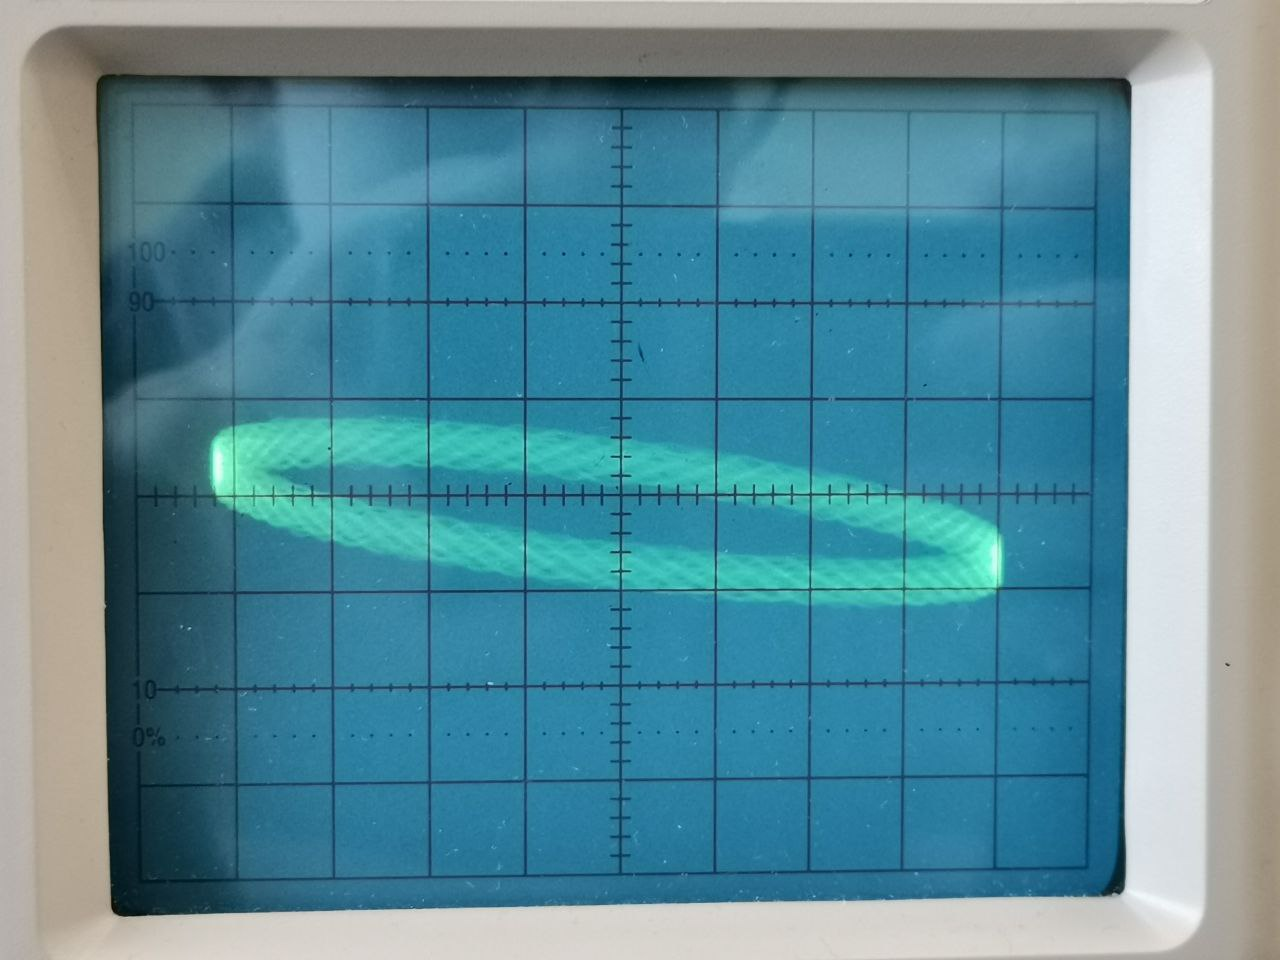
\includegraphics[width=0.9\linewidth]{images/oscl.ellipse5.jpg}\\
            \caption{6.1. Показания осциллографа}
            \label{fig:my_label}
        \end{minipage}%
        \begin{minipage}{.5\textwidth}
            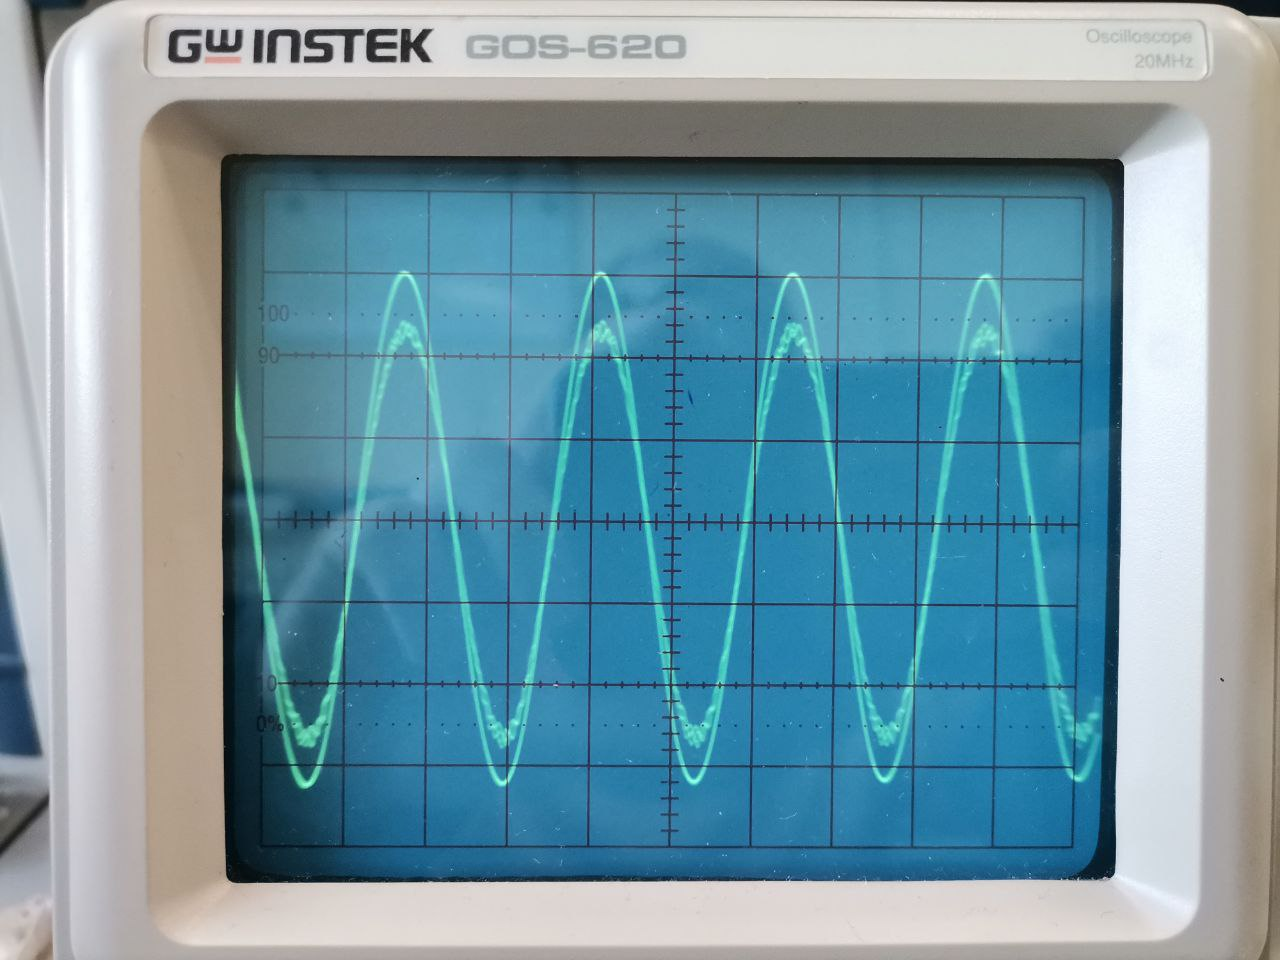
\includegraphics[width=0.9\linewidth]{images/oscl1.jpg}\\
            \caption{6.2. Показания осциллографа}
            \label{fig:my_label}
        \end{minipage}
    \end{figure}
\end{frame}

\begin{frame}{Результаты измерений}
    \begin{figure}[ht]
        \begin{spacing}{0.25}
        \begin{minipage}{.5\textwidth}
            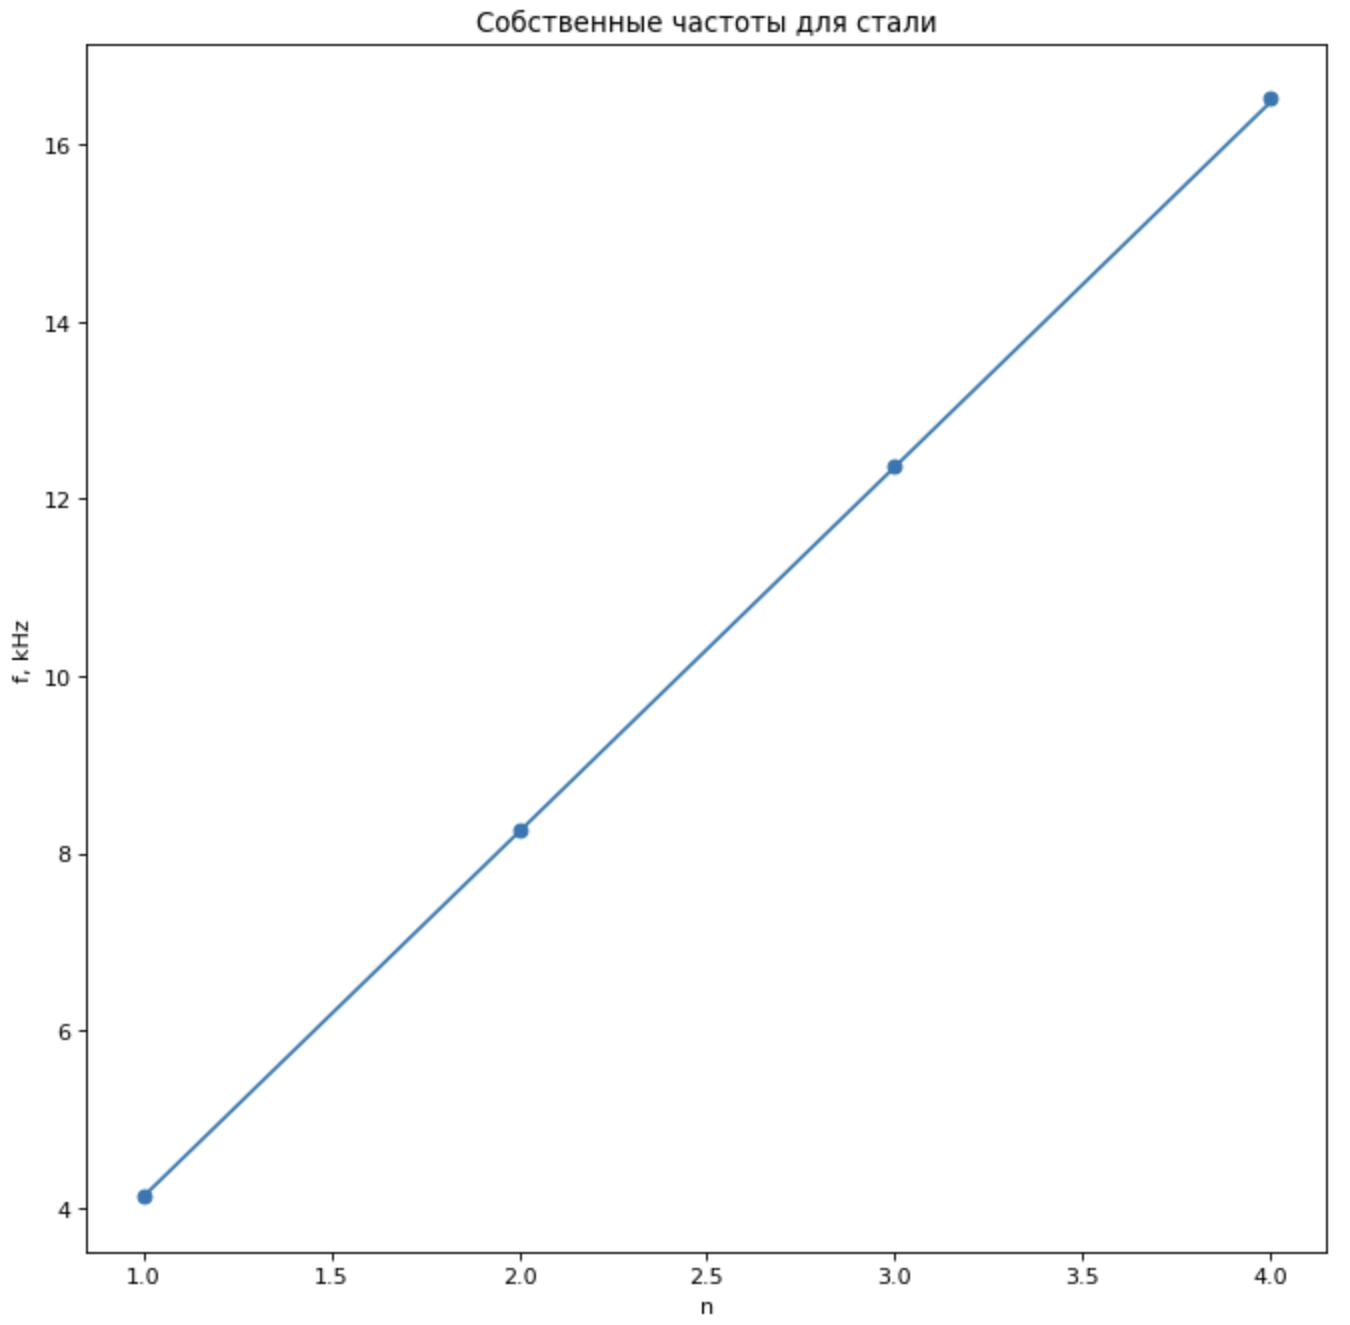
\includegraphics[width=1.0\linewidth]{images/сталь.png}\\
            \caption{7.1}
            \label{fig:my_label}
        \end{minipage}%
        \begin{minipage}{.5\textwidth}
            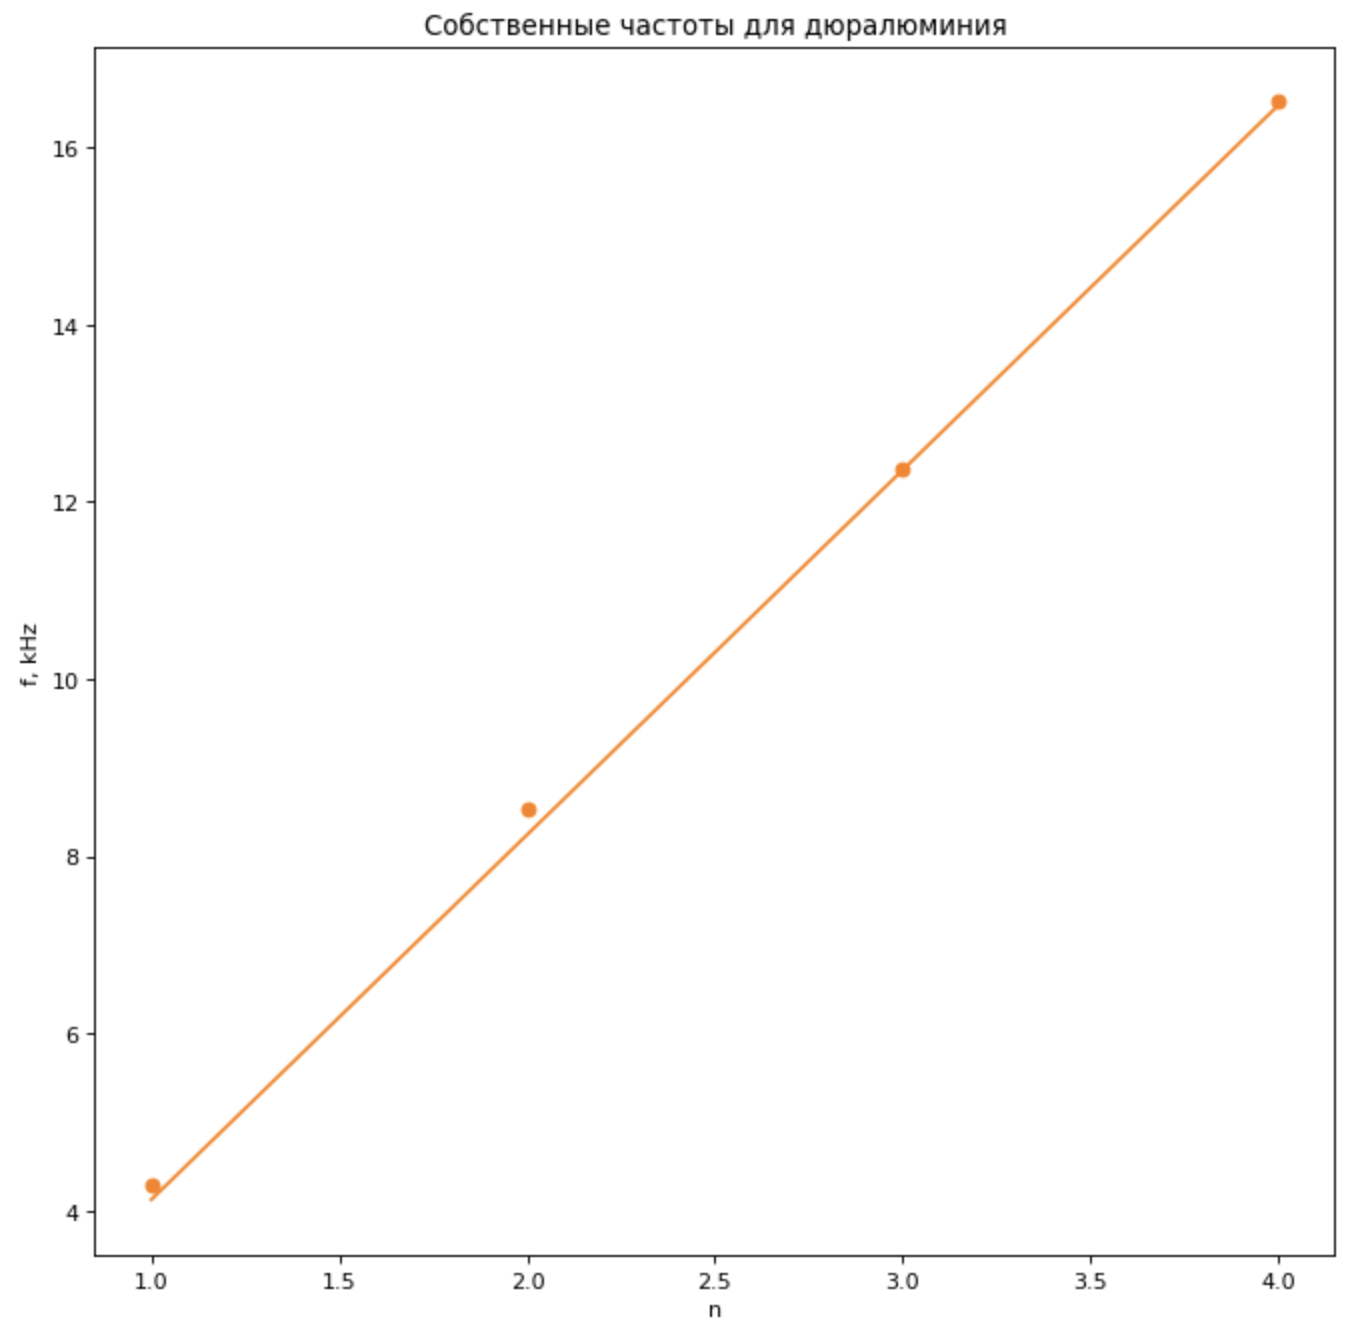
\includegraphics[width=1.0\linewidth]{images/дюралюминий.png}\\
            \caption{7.2}
            \label{fig:my_label}
        \end{minipage}
        \end{spacing}
    \end{figure}
\end{frame}

\begin{frame}{Результаты измерений}
    $$c_{steel} = 4.94 \cdot 10^3 \frac{m}{s}, \;\;\;\;\; c_{duralumin} = 4.94 \cdot 10^3 \frac{m}{s}$$
    $$E = \rho \cdot c^2$$
    $$E_{steel} = 185 \cdot 10^9 \;Pa, \;\;\;\;\; E_{duralumin} = 65 \cdot 10^9 \;Pa$$
\end{frame}

\begin{frame}{Результаты измерений добротности для дюралюминия}
    \begin{figure}
        \centering
        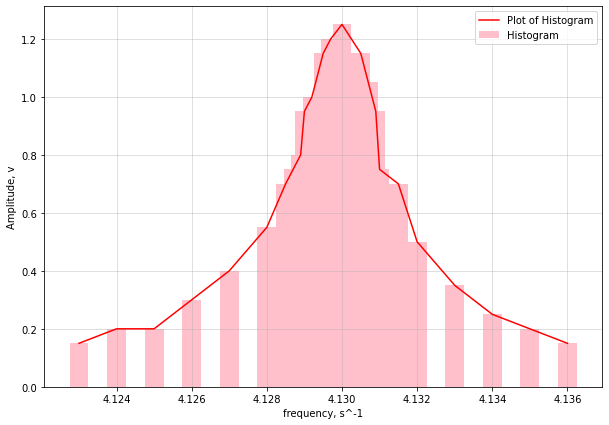
\includegraphics[scale=0.45]{images/Chart1.png}
        \caption{7. График измерения добротности}
        \label{fig:my_label}
    \end{figure}
\end{frame}

\begin{frame}{Результаты измерений добротности для дюралюминия}
    $$Q = \frac{f(A_{max})}{\Delta f}$$
    $$\Delta f = 2 \cdot \bigg(f(A_{max}\bigg) - f\bigg(\frac{A_{max}}{\sqrt{2}}\bigg)\bigg)$$
    $$Q = 2 \cdot 10^3$$
\end{frame}

\begin{frame}{Результаты измерений параметров стержней}
    \begin{table}[t]
        \tabcolsep=0.15cm
        \centering
        \begin{tabular}{|c|c|c|c|c|c|c|c|}
            \hline
            Бебра & m, g & h, cm & D, cm & \rho, \frac{g}{cm^3} & L, cm & E, GPa & c, 10^3 m/s\\ \hline
             Медь & 41 & 4 & 1.2 & 9.2 & 60 & 41 & 3.5\\
             Сталь & 35 & 4 & 1.2 & 7.7 & 60 & 35 & 5.1\\ 
             Алюминий & 12 & 4 & 1.19 & 2.7 & 60 & 12 & 5.1\\ 
            \hline
        \end{tabular}
        \caption{Табл 1.}
        \label{tab:my_label}
    \end{table}
\end{frame}

\begin{frame}{Результаты измерений добротности для дюралюминия}
    \begin{figure}[ht]
        \begin{minipage}{.5\textwidth}
            \begin{table}
                \tabcolsep = 0.15cm
                \centering
                \begin{tabular}{|c|c|c|}
                    \hline
                    $$f, kHz$$ & A, DIV & A, V \\
                    \hline
                    4.123 & 0.3	& 1.24 \\ 
                    4.124 & 0.4	& 1.65 \\ 
                    4.125 &	0.4	& 1.65 \\
                    4.126 &	0.6	& 2.48 \\
                    4.127 &	0.8	& 3.30 \\
                    4.127 &	1.1	& 4.54 \\
                    4.128 &	1.4	& 5.78 \\
                    4.128 &	1.5	& 6.19 \\
                    4.128 &	1.6	& 6.61 \\
                    4.129 &	1.9	& 3.61 \\
                    4.129 &	2.0	& 3.80 \\
                    4.129 &	2.3	& 4.37 \\
                    \hline
                \end{tabular}
            \end{table}
        \end{minipage}%  
        \begin{minipage}{.5\textwidth}
            \begin{table}
                \tabcolsep = 0.15cm
                \centering
                \begin{tabular}{|c|c|c|}
                    \hline
                    $$f, kHz$$ & A, DIV & A, V \\
                    \hline
                    4.139 &	2.4	& 4.56 \\
                    4.130 &	2.5	& 10.32 \\
                    4.131 &	2.3	& 9.50 \\
                    4.131 &	2.1	& 8.67 \\
                    4.131 &	1.9	& 7.85 \\
                    4.131 &	1.5	& 6.20 \\ 
                    4.132 &	1.4	& 5.78 \\
                    4.132 &	1.0	& 4.13 \\
                    4.133 &	0.7	& 2.89 \\
                    4.134 &	0.5	& 2.07 \\
                    4.135 &	0.4 & 1.65 \\
                    4.136 & 0.3	& 1.24 \\
                    \hline
                \end{tabular}
            \end{table}
        \end{minipage}
    \end{figure}
\end{frame}

\end{document}